\documentclass[11pt]{article}
\usepackage[T1]{fontenc}
\usepackage{lmodern}
\usepackage[margin=1in]{geometry}
\usepackage{amsmath,amssymb,booktabs,array,graphicx,xcolor,tikz}
\usetikzlibrary{arrows.meta,positioning}
\usepackage{caption,enumitem,microtype,longtable,listings}
\usepackage[hidelinks]{hyperref}
\captionsetup{font=small,labelfont=bf}
\setlength{\parskip}{0.3em}
\setlength{\emergencystretch}{3em}
\newcommand{\code}[1]{\texttt{\small #1}}
\lstset{basicstyle=\ttfamily\footnotesize,breaklines=true,columns=fullflexible,keepspaces=true,frame=single}
\title{\bfseries LLM-Enhanced Process-Aware Knowledge Tracing\\from Student Solution Steps for Concept Deficiency Prediction}
\author{Temesgen\\[2pt]\normalsize University of Vienna}
\date{September 2026}
\newcommand{\FoneA}{24.28}
\newcommand{\FoneB}{27.39}
\newcommand{\FoneC}{32.06}

\begin{document}
\maketitle
\begin{abstract}
Knowledge tracing usually predicts correctness; concept deficiency prediction instead asks which mathematical concepts a student will fail to apply. We investigate an offline Gemini analyzer that converts past solutions into missing-concept signals, error types and summary embeddings, followed by a small two-head LSTM. We use the official MathEDU/ConceptKT split of 3,644 training and 404 test interactions from six students. A revision audit identified an occurrence-key bug that overwrote labels for repeated problem IDs, including one training record with a later test occurrence's labels. All experiments reported here were rerun after correcting this bug. Across five seeds, macro-F1 over 13 categories is \FoneA\% for the correctness-only baseline, \FoneB\% for full analyzer features and \FoneC\% for gold past features. We report all feature subsets, paired uncertainty, per-category support, calibration, and six leave-one-student-out folds. The expanded analyzer check covers 87 incorrect validation answers and finds 50.6\% error-type agreement, substantially below the original 20-record spot check. Results are exploratory evidence on six fixed students; seed variability and weak analyzer agreement limit conclusions about reliable generalization.
\end{abstract}

\section{Introduction}
Knowledge tracing (KT) models students' evolving knowledge from interaction histories. Deep Knowledge Tracing uses a recurrent model to predict future correctness \cite{piech2015dkt}. Correctness alone discards evidence in worked solutions about misconceptions and partial understanding. Process-aware KT \cite{huang2024remembering,park2025statuskt} and text-aware KT \cite{lee2024lkt,ozyurt2024kcqrl} motivate extracting that evidence. ConceptKT \cite{kang2026conceptkt} supplies a more diagnostic target: deficiencies among 55 mathematical concepts grouped into 13 categories.

Our research question is: \emph{Can LLM-derived process signals from past student solutions improve future concept deficiency prediction over a correctness-only baseline?} The LLM describes completed work offline; a small recurrent model predicts the next interaction. The contributions are:
\begin{itemize}[leftmargin=1.4em,itemsep=2pt]
\item Offline extraction of structured LLM process signals with cached outputs and an explicit past-only feature boundary.
\item A compact two-head LSTM that consumes only preceding interactions and masks deficiency outputs to the next question's associated concepts.
\item A controlled A/B/C comparison with a gold-feature reference and all seven nonempty subsets of the three analyzer signals.
\item A reproducible evaluation pipeline with occurrence-safe feature keys, causality tests, saved predictions, seed uncertainty, and student-level diagnostics.
\end{itemize}
The corrected results replace the earlier draft's numbers. A higher mean is not sufficient evidence of a reliable gain: five optimizer seeds on six students do not represent five independent student populations.

\section{Related Work}
DKT \cite{piech2015dkt} established recurrent modeling of correctness histories. Process-oriented work distinguishes recalling a concept from applying it in a solution \cite{huang2024remembering}. Language-model KT \cite{lee2024lkt} and concept-aligned question representations \cite{ozyurt2024kcqrl} provide ways to incorporate semantic information. StatusKT extracts mathematical-proficiency representations from solution processes for downstream KT \cite{park2025statuskt}; our work follows this intermediate-feature approach with a deliberately smaller model and a different diagnostic output.

MathEDU \cite{hsu2026mathedu} provides worked solutions and teacher annotations. ConceptKT \cite{kang2026conceptkt} adds concept deficiency labels and evaluates history-based LLM prediction. The internal A/B/C comparison here uses a common split, model family, loss and threshold protocol. Published ConceptKT scores are contextual rather than a head-to-head benchmark: their inference setup differs, and 55-concept F1 cannot be compared directly with our coarser 13-category F1. Reproducible split handling is especially important in KT, as emphasized by pyKT \cite{liu2022pykt}.

\section{Data and Preprocessing}
ConceptKT provides a chronological spine of 4,048 records from six students; MathEDU supplies the worked solution, final answer, correctness and teacher error annotation. Their composite-key join on \code{(id, student\_id)} covers all 4,048 records. Problem IDs are identifiers, not timestamps: order follows the ConceptKT file within each student. We retain the official 3,644/404 split. The last 10\% (rounded, at least one) of each student's training history forms validation. The first interaction of each student is history only.

The corpus has 3,050 correct and 998 incorrect answers; 463 records have nonempty gold deficiency. Gold targets and associated concepts use the canonical 55-concept taxonomy. Missing labels are converted to empty lists and only canonical concepts are retained. MathEDU contains no question text in this run, so the analyzer reads the solution, answer and known correctness. Its prompt does not contain teacher errors or gold missing concepts.

\subsection{Duplicate occurrences and the corrected feature store}
The MathEDU lookup joins process fields by composite key. ConceptKT contains two repeated composite keys with different concept annotations. They cannot safely be assumed to be identical records or verified re-attempts. For each key occurring $k$ times in the official test file, the final $k$ occurrences in the spine are marked test; both occurrences remain in the dataset. The feature store now uses \code{(student\_id, seq\_pos)} so labels, masks and history features retain occurrence identity.

For a concrete masked example, student S* has problem Q* at zero-based positions 573 (train) and 649 (test). The earlier occurrence is annotated with \emph{Mixed Solution Concentration}; the later one with \emph{Basic Math Operations}. Previously the shared feature-store key replaced the earlier occurrence with the later vector. The corrected store preserves both. Another repeated key occurs at positions 673 and 677 within a different student's test tail: its labels are \emph{Arithmetic Mean} and \emph{Compound Interest}. Correcting these restores a category positive from Finance to Statistics and Probability. The total remains 59 positive concept labels. Because the process join is still keyed by problem/student, these source annotation disagreements remain a data-quality limitation; we do not invent distinct solutions for them.

\subsection{Error normalization}
We use the first teacher-review error annotation. Table~\ref{tab:mapping} gives every raw-to-final mapping; absent errors map to \code{none}. Unknown strings also map to \code{none} in the current loader, so taxonomy changes need an explicit audit. Comprehension-to-concept and measurement-to-calculation are interpretive decisions, not universally interchangeable labels.
\begin{table}[htbp]\centering\small
\caption{Exact eight-string normalization; the sixth final type, none, covers absent errors.}\label{tab:mapping}
\begin{tabular}{@{}p{.49\linewidth}p{.45\linewidth}@{}}\toprule
Raw MathEDU string & Final type\\\midrule
Wrong mathematical operation/concept & wrong\_operation\_or\_concept\\
Comprehension error & wrong\_operation\_or\_concept\\
Lack of necessary mathematical concepts & lack\_of\_concepts\\
Unfinished answer & incomplete\_answer\\
Arithmetical error & calculation\_error\\
Algebraic error & calculation\_error\\
Careless error & careless\_error\\
Measurement error & calculation\_error\\\bottomrule
\end{tabular}\end{table}

\section{Method}
Figure~\ref{fig:pipeline} summarizes the offline extraction boundary and the two prediction heads. No analyzer API call occurs during the revision experiments: an incomplete cache raises an error before feature construction.
\begin{figure}[htbp]\centering
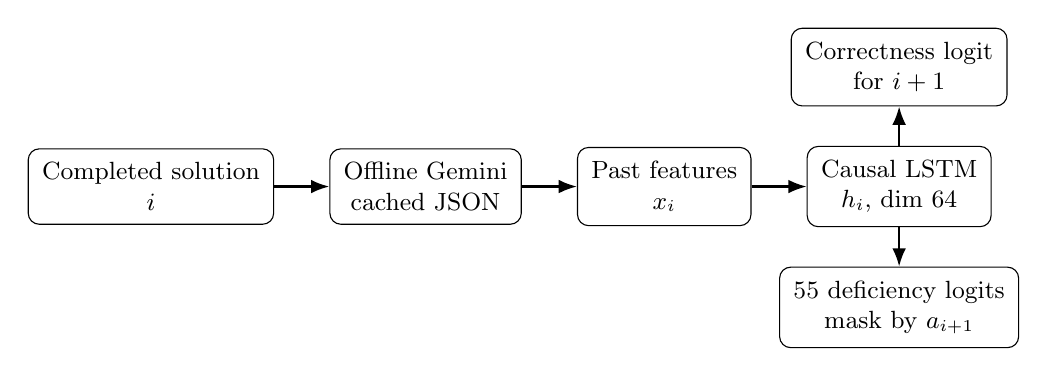
\begin{tikzpicture}[node distance=5mm and 7mm,box/.style={draw,rounded corners,align=center,font=\small,inner sep=5pt},arr/.style={-{Latex},thick}]
\node[box] (past) {Completed solution\\$i$};
\node[box,right=of past] (llm) {Offline Gemini\\cached JSON};
\node[box,right=of llm] (vec) {Past features\\$x_i$};
\node[box,right=of vec] (lstm) {Causal LSTM\\$h_i$, dim 64};
\node[box,below=of lstm] (def) {55 deficiency logits\\mask by $a_{i+1}$};
\node[box,above=of lstm] (cor) {Correctness logit\\for $i+1$};
\draw[arr](past)--(llm);\draw[arr](llm)--(vec);\draw[arr](vec)--(lstm);
\draw[arr](lstm)--(def);\draw[arr](lstm)--(cor);
\end{tikzpicture}
\caption{Two-head sequence model. The next question's associated concepts are known metadata; its answer, solution and deficiencies are not visible to $h_i$.}\label{fig:pipeline}
\end{figure}

\subsection{Analyzer and feature encoding}
The cached analyzer model is \code{gemini-3.1-flash-lite}, using temperature zero and a Pydantic JSON schema. Temperature zero does not guarantee identical responses across provider versions; the fixed cache makes downstream comparisons repeatable. The prompt requests associated concepts, missing concepts, one of six error types, a faulty step, partial understanding, and a short process summary. Sanitation removes out-of-taxonomy concepts and forces empty missing concepts and error type \code{none} when the supplied correctness is true. Agreement on correct cases would therefore be tautological; our expanded check uses wrong answers.

The cache key is SHA-256 of prompt version, model name and user prompt. It does not directly hash the system instruction, so changing that instruction requires a prompt-version bump. The archived cache has 3,962 files covering all interactions. The original log records 3,882 extraction API calls; this is a historical run count, not a count of calls made for these revisions. Cache presence is mandatory here; no malformed-output fallback was needed in the rerun.

Table~\ref{tab:features} defines model inputs. The summary encoder is frozen \code{all-MiniLM-L6-v2} \cite{reimers2019sbert}. Its 384-dimensional output is L2-normalized and concatenated directly: there is \emph{no projection layer or projection activation}. Empty text is replaced with a space and encoded, not replaced by a zero vector. Arm C alone uses an explicit zero summary block to preserve the original B/C dense layout.
\begin{table}[htbp]\centering\small
\caption{Feature components; the associated-concept mask always comes from gold question metadata.}\label{tab:features}
\begin{tabular}{@{}lll@{}}\toprule
Component & Dimension & Source / arm\\\midrule
Associated concepts + correctness & $55+1$ & Gold metadata and grading, all\\
Missing concepts (M) & 55 & Analyzer B; gold C\\
Error type (E) & 8 learned & Analyzer B; gold C\\
Summary (S) & 384 frozen & Analyzer B; zero block C\\\bottomrule
\end{tabular}\end{table}

\paragraph{End-to-end example (IDs masked).}
A real cached solution states $9<a\leq21$, $19<b<31$, then incorrectly concludes $21/19\leq a/b<31/9$. Its analyzer output is shown below (the faulty expression uses equivalent plain mathematical notation for readability).
\begin{lstlisting}
{
 "associated_concepts": ["Range of Values"],
 "missing_concepts": ["Range of Values"],
 "error_type": "wrong_operation_or_concept",
 "faulty_step": "21/19 <= a/b < 31/9",
 "partial_understanding": ["The student understands that the bounds of a quotient can be determined by the bounds of the numerator and denominator."],
 "process_summary": "The student incorrectly combined the bounds of two variables to determine the range of their quotient, failing to account for the correct extreme values of the fraction."
}
\end{lstlisting}
In the canonical zero-based taxonomy, \emph{Range of Values} is index 3. Thus this record's associated mask and LLM missing vector both have only entry 3 set, correctness is 0, error ID is 0, and the 384-dimensional summary has norm 1.000. Its B input has $55+1+55+384+8=503$ dimensions. This record's mask is used when it is the target; its features are available only when predicting its successor. The exact cached JSON and solution are saved in \code{results/revisions/feature\_example.json}.

\subsection{Architecture, loss, masking and threshold selection}
Let $x_i$ encode completed interaction $i$, $h_i=\operatorname{LSTM}(x_i,h_{i-1})$, and $a_{i+1,c}$ indicate whether concept $c$ is associated with the next question. After output dropout ($0.4$), linear heads produce correctness logit $u_i$ and deficiency logits $z_{i,c}$. The single-layer hidden size is 64. Masking is explicit:
\begin{equation}
\tilde z_{i,c}=\begin{cases}z_{i,c},&a_{i+1,c}=1,\\-10^9,&a_{i+1,c}=0,\end{cases}
\qquad p_{i,c}=\sigma(\tilde z_{i,c}).
\end{equation}
For gold deficiency $y_{i+1,c}$, define $p^{\star}_{i,c}=y_{i+1,c}p_{i,c}+(1-y_{i+1,c})(1-p_{i,c})$. Over a student's selected training target positions $I$, the implemented focal binary cross-entropy is
\begin{align}
\ell_{i,c}&=-y_{i+1,c}\log p_{i,c}-(1-y_{i+1,c})\log(1-p_{i,c}),\\
L_D&=\frac{\sum_{i\in I,c}a_{i+1,c}\,[\max(1-p^{\star}_{i,c},10^{-6})]^2\ell_{i,c}}
{\sum_{i\in I,c}a_{i+1,c}},\\
L&=\frac{1}{|I|}\sum_{i\in I}\operatorname{BCEWithLogits}(u_i,r_{i+1})+L_D.
\end{align}
BCE is evaluated numerically with logits. Only associated entries contribute; an empty mask contributes zero. This is the focal modulation of Lin et al.\ \cite{lin2017focal}, with $\gamma=2$, \emph{no additional alpha/class weights}, and equal weights for correctness and deficiency losses. Each student sequence produces one optimizer step, so students are not implicitly weighted by their number of concepts through a pooled loss.

After choosing the checkpoint with lowest mean student validation loss, we select a single threshold per arm/seed:
\begin{equation}
\tau^{\star}=\underset{\tau\in\{.10,.15,.20,.25,.30,.35,.40,.50\}}{\arg\max}
\operatorname{MacroF1}_{13}(Y_{val},\mathbb{1}[P_{val}\geq\tau]).
\end{equation}
Concept indicators are OR-aggregated into categories before category F1. Ties select the lowest grid threshold; a validation set with no positive labels falls back to $.50$. Test labels never select a threshold. Figure~\ref{fig:threshold} shows the flow.
\begin{figure}[htbp]\centering
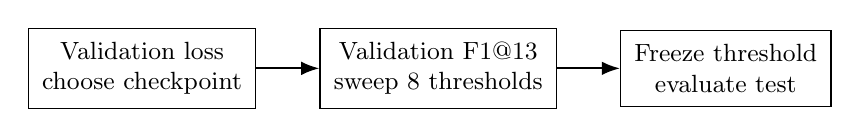
\begin{tikzpicture}[node distance=8mm,box/.style={draw,align=center,font=\small,inner sep=5pt},arr/.style={-{Latex},thick}]
\node[box](v){Validation loss\\choose checkpoint};
\node[box,right=of v](t){Validation F1@13\\sweep 8 thresholds};
\node[box,right=of t](f){Freeze threshold\\evaluate test};
\draw[arr](v)--(t);\draw[arr](t)--(f);
\end{tikzpicture}
\caption{Checkpoint and threshold selection use validation only.}\label{fig:threshold}
\end{figure}

\subsection{Causality checks}
When predicting target position $p+1$, only inputs $0,\ldots,p$ may affect its hidden state. The runtime check in \code{src/dataset.py} is equivalent to:
\begin{lstlisting}
for p, target in enumerate(target_positions):
    visible = input_positions[:p + 1]
    assert target not in visible
    assert all(v < target for v in visible)
\end{lstlisting}
The following tests guard index alignment, occurrence identity, and actual model causality, respectively:
\begin{lstlisting}
test_assert_no_leakage_fires_when_target_in_history
test_duplicate_problem_ids_preserve_occurrence_labels
test_target_and_future_features_cannot_change_current_prediction
\end{lstlisting}
 The old index check alone did not detect overwritten features; the added tests close that gap. Later test interactions may use earlier completed test answers as history, an online rolling-history protocol with fixed model weights.

\section{Experimental Setup}
\paragraph{Arms and ablations.}
A uses associated concepts and correctness. B adds analyzer M, E and S; C adds gold past missing concepts and gold past error types. We run M, E, S, ME, MS and ES separately in addition to full MES (B). Absent components are physically removed in ablations; this changes parameter counts, which we report. C retains its zero summary block from the original architecture. Consequently C is a gold-feature reference, not a guaranteed mathematical ceiling: it lacks summary information and need not outperform B in every run.

\paragraph{Fixed hyperparameters and rationale.}
We retain hidden size 64, output dropout 0.4, Adam learning rate $10^{-3}$, maximum 60 epochs and early-stop patience 8. A compact state and appreciable regularization limit capacity given six students; $10^{-3}$ is the original conventional Adam starting value. These are pragmatic prototype choices, not validated optima. No archived hyperparameter search supports a claim of optimality, and no retrospective search was conducted for this revision. Keeping them fixed isolates feature changes and avoids selecting configurations from the exposed test results. A larger backbone is not proven to overfit merely because the sample is small.

\paragraph{Uncertainty and metrics.}
Seeds are $\{0,1,2,3,4\}$, matched across arms. We report population standard deviation across these five observations (matching the original convention) and a 95\% Student-$t$ interval for the seed mean, $\bar f\pm t_{.975,4}s/\sqrt5$, where $s$ is the sample standard deviation. The paired differences B$-$A and C$-$B receive two-sided paired $t$-tests and exact sign-flip tests over all $2^5$ sign assignments, with Bonferroni adjustment for these two comparisons. Seed-pair exchangeability and approximate normality for the $t$ test are assumptions; neither test measures uncertainty over new student populations. The smallest two-sided exact $p$ with five nonzero pairs is $2/32=.0625$.

Macro-F1 includes all 55 concepts or all 13 categories, with zero for undefined category F1. Per-category counts are category-positive \emph{interactions}, whereas 59 is a concept-label count. Error breakdowns are one-vs-rest TP/FP/FN/TN, appropriate for multilabel targets. Calibration uses ten equal-width probability bins on associated concept entries only:
$\mathrm{ECE}=\sum_b(n_b/N)|\overline p_b-\overline y_b|$; Brier score is $N^{-1}\sum(p-y)^2$. Structural masked zeros are excluded so they do not make calibration appear artificially good.

\paragraph{Per-student and LOSO protocol.}
For each arm we summarize each student's official test tail under the five-seed chronological model. We also train six LOSO folds at seed 0 with unchanged hyperparameters: five students supply training and validation, and the held student's data never selects weights, epochs or thresholds. The held student's observed history is available for recurrent inference on their official test tail. This measures transfer to an unseen student with observed history, not cold start. We report folds individually and pool their out-of-fold test predictions; a mean over fold macro-F1 is a different estimand.

\section{Results}
\subsection{Analyzer--gold agreement}
The expanded study is a census of all 87 wrong, gold-error-annotated answers in the actual validation tails, rather than the first 20 eligible corpus records used previously. Students contribute 15, 4, 18, 16, 21 and 13 examples. Error-type agreement is $44/87=50.6\%$; Table~\ref{tab:analyzer} reports every normalized class. The earlier $15/20=75\%$ spot check did not represent the validation population. In particular, the analyzer fails to recover several minority classes.
\begin{table}[htbp]\centering\small
\caption{Error-type agreement on all 87 annotated wrong validation answers. Undefined precision/recall is reported as zero.}\label{tab:analyzer}
\begin{tabular}{@{}lrrr@{}}\toprule
Gold class & Support & Precision & Recall\\\midrule
Wrong operation/concept & 54 & 0.695 & 0.759\\
Lack of concepts & 11 & 0.000 & 0.000\\
Calculation & 8 & 0.176 & 0.375\\
Incomplete answer & 13 & 0.000 & 0.000\\
Careless & 1 & 0.000 & 0.000\\
None & 0 & 0.000 & 0.000\\
\bottomrule\end{tabular}\end{table}

Among the 45 validation records with nonempty gold deficiency (49 gold concept labels), concept-level micro precision is 27.0\% and recall is 20.4\%. These scores compare exact canonical concepts without filtering analyzer predictions by the gold mask. Conditioning on gold-positive records excludes false alarms on gold-negative cases, so precision is conditional, not a whole-validation diagnostic rate. The appendix reports individual concept support and precision/recall plus the six-way error confusion matrix. The taxonomy mapping and incomplete problem context are plausible sources of disagreement; this study cannot distinguish model mistakes from gold annotation ambiguity.

\subsection{Corrected primary comparison and uncertainty}
Table~\ref{tab:main} reports the corrected official-split results; Table~\ref{tab:significance} gives paired uncertainty. All values are recomputed from saved predictions after the occurrence-key fix.
\begin{table}[htbp]\centering\small
\caption{Corrected official test results. Percent except AUC; F1@13 includes seed SD and a 95\% seed-mean interval.}\label{tab:main}
\begin{tabular}{@{}lrrrrrrr@{}}\toprule
Arm & Acc. & AUC & F1@55 & F1@13 $\pm$ SD & 95\% CI & P@13 & R@13\\\midrule
A & 71.78 & 0.602 & 10.12 & 24.28 $\pm$ 3.92 & [18.84, 29.71] & 20.41 & 39.81\\
B & 71.78 & 0.587 & 11.58 & 27.39 $\pm$ 5.03 & [20.41, 34.36] & 26.31 & 41.28\\
C & 71.78 & 0.595 & 13.70 & 32.06 $\pm$ 1.94 & [29.38, 34.75] & 29.73 & 48.88\\
\bottomrule\end{tabular}\end{table}

\begin{table}[htbp]\centering\small
\caption{Paired F1@13 differences in percentage points. Two-sided tests; final column adjusts the two paired $t$ comparisons. Exact tests also receive Bonferroni adjustment in JSON.}\label{tab:significance}
\begin{tabular}{@{}lrrrrr@{}}\toprule
Pair & $\Delta$ & 95\% CI ($\Delta$) & $p_t$ & $p_{exact}$ & $p_{t,adj}$\\\midrule
B$-$A & 3.11 & [-8.38, 14.61] & 0.494 & 0.5625 & 0.988\\
C$-$B & 4.68 & [-3.43, 12.79] & 0.185 & 0.2500 & 0.369\\
\bottomrule\end{tabular}\end{table}

B changes mean F1@13 by +3.11 percentage points relative to A. The paired $t$ test gives $p=0.494$ (two-comparison adjusted $p=0.988$), and the exact sign-flip test gives $p=0.5625$. Neither primary comparison establishes a statistically reliable gain at the 5\% level under the exact test. Mean ordering must not be described as an ordering that holds for every seed, or as proof that the gain is independent of thresholding.

The original A/B/C numbers are retained under \code{results/historical/}, but cannot substantiate a leakage-safe result because the old feature store overwrote occurrence labels. Differences from the draft also reflect the recorded current Python/PyTorch environment, so a numerical change cannot be attributed exclusively to the bug fix.

\subsection{Which analyzer signals matter?}
Table~\ref{tab:ablations} reports every nonempty signal subset and its macro-F1@13 change from A on the same split and seeds. Comparing full B with ME directly quantifies removal of the summary. These are controlled feature-removal experiments under one architecture, not estimates of a signal's intrinsic causal value: input dimensionality, learned capacity and optimization also change.
\begin{table}[htbp]\centering\small
\caption{All signal subsets on the same five seeds and official split. M: missing concepts; E: error type; S: summary. Parameters include the allocated error embedding, even where unused.}\label{tab:ablations}
\begin{tabular}{@{}lrrrr@{}}\toprule
Inputs & F1@13 & SD & $\Delta$ vs A (pp) & Parameters\\\midrule
A & 24.28 & 3.92 & +0.00 & 34920\\
A + M & 23.29 & 1.65 & -0.98 & 49000\\
A + E & 32.00 & 1.73 & +7.73 & 36968\\
A + S & 23.61 & 1.18 & -0.67 & 133224\\
A + M + E & 29.98 & 3.46 & +5.70 & 51048\\
A + M + S & 22.97 & 1.21 & -1.31 & 147304\\
A + E + S & 25.56 & 2.87 & +1.29 & 135272\\
A + M + E + S (B) & 27.39 & 5.03 & +3.11 & 149352\\
Gold M + E (C) & 32.06 & 1.94 & +7.79 & 149352\\
\bottomrule\end{tabular}\end{table}

The highest exploratory mean among analyzer variants is A + E (32.00\%). Removing summary from full B changes F1@13 by +2.59 points (ME 29.98\% versus MES 27.39\%). The full feature bundle is therefore not automatically preferable. These contrasts share the exposed test set; they characterize this prototype and should be validated independently before selecting a production variant.


\subsection{Category support and error breakdowns}
Table~\ref{tab:categories} includes all 13 categories and their positive test interaction counts; zero-support categories remain in the macro average. The appendix gives mean TP/FP/FN/TN across seeds, preserving each seed's own validation-selected threshold. Sparse categories can change substantially when only one or two predictions change. Aggregate category improvements do not establish that the analyzer correctly diagnosed individual test errors.
\begin{table}[htbp]\centering\small
\caption{All-category F1 with positive test interaction support. F1 is a proportion and averaged over seeds.}\label{tab:categories}
\begin{tabular}{@{}lrrrrr@{}}\toprule
Category & Positives & A & B & C & $\Delta$ B$-$A\\\midrule
Basic Arithmetic & 9 & 0.000 & 0.000 & 0.019 & +0.000\\
Prime Numbers & 2 & 0.391 & 0.365 & 0.402 & -0.026\\
Factors and Multiples & 0 & 0.000 & 0.000 & 0.000 & +0.000\\
Physics & 6 & 0.214 & 0.246 & 0.431 & +0.032\\
Ratio and Proportion & 7 & 0.000 & 0.000 & 0.067 & +0.000\\
Finance & 8 & 0.446 & 0.438 & 0.429 & -0.008\\
Statistics and Probability & 8 & 0.000 & 0.044 & 0.323 & +0.044\\
Polynomials & 1 & 0.467 & 0.467 & 0.427 & +0.000\\
Sequences and Series & 2 & 0.114 & 0.520 & 0.640 & +0.406\\
Geometry & 8 & 0.533 & 0.534 & 0.486 & +0.001\\
Set Theory & 1 & 0.133 & 0.089 & 0.089 & -0.044\\
Permutations and Combinations & 6 & 0.857 & 0.857 & 0.857 & +0.000\\
Other & 0 & 0.000 & 0.000 & 0.000 & +0.000\\
\bottomrule\end{tabular}\end{table}

The largest B$-$A category change is Sequences and Series ($+0.406$ F1), but it has only two positive test interactions. Statistics and Probability rises by $0.044$ with eight positives; Set Theory drops by $0.044$ with one positive, and Prime Numbers drops by $0.026$ with two. These counts argue against a broad topic-level explanation from the category means alone.

\subsection{Per-student transfer and calibration}
Table~\ref{tab:students} reports chronological per-student mean F1 and seed-0 LOSO F1, with support. Table~\ref{tab:losopooled} compares pooled LOSO predictions to the matching seed-0 chronological models. These limited folds cannot establish population generalization.
\begin{table}[htbp]\centering\small
\caption{Per-student F1@13 (percent): chronological means over five seeds, LOSO at seed 0. Pos. counts concept labels.}\label{tab:students}
\begin{tabular}{@{}lrrrrrrrr@{}}\toprule
Student & Targets & Pos. & A & B & C & LOSO A & LOSO B & LOSO C\\\midrule
S1 & 68 & 8 & 7.69 & 7.69 & 7.69 & 7.69 & 0.00 & 7.69\\
S2 & 68 & 4 & 1.54 & 1.54 & 2.56 & 0.00 & 0.00 & 0.00\\
S3 & 68 & 10 & 10.00 & 9.23 & 9.23 & 7.69 & 16.03 & 18.28\\
S4 & 66 & 8 & 13.53 & 13.42 & 13.40 & 15.85 & 15.85 & 13.29\\
S5 & 68 & 19 & 27.41 & 32.48 & 40.87 & 40.64 & 28.39 & 38.46\\
S6 & 66 & 10 & 18.67 & 17.44 & 17.86 & 19.57 & 19.96 & 16.61\\
\bottomrule\end{tabular}\end{table}

\begin{table}[htbp]\centering\small
\caption{Pooled LOSO predictions versus matched chronological seed 0 (F1@13 percent); all 404 test targets.}\label{tab:losopooled}
\begin{tabular}{@{}lrrr@{}}\toprule
Arm & Chronological seed 0 & Pooled LOSO & Difference (pp)\\\midrule
A & 22.93 & 25.70 & +2.76\\
B & 23.64 & 24.43 & +0.79\\
C & 31.14 & 31.08 & -0.06\\
\bottomrule\end{tabular}\end{table}

Pooling the held-student test predictions gives A=25.70\%, B=24.43\% and C=31.08\%. Individual student scores vary substantially; a pooled score is not evidence that every student benefits. The LOSO folds share training students, so their six results are dependent and are not treated as six independent significance-test observations.

Table~\ref{tab:calibration} reports associated-entry ECE and Brier scores. Scores have not been probability-calibrated; the focal objective and threshold tuning optimize discrimination, not probability accuracy. The appendix lists every selected threshold, and the complete reliability bins are in each run's diagnostic JSON.
\begin{table}[htbp]\centering\small
\caption{Associated-entry calibration on the test set, mean over five seeds. Lower ECE and Brier are better; no post-hoc probability calibration was fitted.}\label{tab:calibration}
\begin{tabular}{@{}lrrr@{}}\toprule
Arm & Entries per seed & ECE & Brier\\\midrule
A & 511 & 0.1803 & 0.1267\\
B & 511 & 0.1789 & 0.1255\\
C & 511 & 0.1798 & 0.1252\\
\bottomrule\end{tabular}\end{table}


\section{Discussion and Threats to Validity}
The corrected experiment yields a mean B$-$A difference of +3.11 F1@13 points. This is a conditional empirical result for a fixed tiny corpus, not a general proof that offline LLM signals improve KT. The feature subsets show why a bundled comparison alone is insufficient, and the expanded agreement study reveals substantial analyzer noise. A gold-feature reference measures one alternative input condition; it cannot quantify an assured amount of recoverable headroom. In particular, a percentage of the A-to-C gap should not be interpreted as the fraction of knowledge captured by the analyzer.

\subsection{Threats to validity}
\paragraph{Internal validity.}
The overwritten-duplicate bug shows why index checks alone were insufficient. Occurrence keys, perturbation tests, fixed splits and cache-only experiments improve control, but conflicting source annotations remain. All arms share a procedure, not equal parameter counts. Validation is reused for stopping and threshold selection, and ablations are exploratory; no best ablation is promoted as a test-selected final model. Hardware/library changes can alter optimization despite fixed seeds.
\paragraph{Construct validity.}
Gold missing concepts are sparse annotations of observed work, not a complete measure of knowledge. The eight-to-six mapping merges distinct error types. No question text is available, and known correctness constrains analyzer output. Gold associated concepts at target time are an oracle metadata assumption that real deployments must satisfy. Category OR aggregation can hide fine-grained errors; zero-support categories depress macro-F1. C has access to gold past features but no summary, so it is not a guaranteed upper bound.
\paragraph{External validity.}
Only six students and 59 positive test concept labels constrain generalization. Seed confidence intervals cover optimizer variability on this fixed corpus, not student sampling. LOSO uses one seed per fold and observed student history. One prompt, one cached LLM and one summary encoder do not establish robustness to analyzer changes, schools, languages or tasks. No live classroom outcome is measured.

\paragraph{Future work.}
Priorities are resolving duplicate source annotation conflicts, collecting more students and diagnostic labels, auditing error normalization with educators, and testing prompt/model sensitivity with complete question text. A validation-only hyperparameter study, alternative KT backbones, and calibrated probabilities are subsequent steps. Feature fusion should be compared under matched parameter budgets before attributing changes entirely to particular signals.

\section{AI Usage}
Gemini (\code{gemini-3.1-flash-lite}) was used as the offline process analyzer. It received completed student solutions, final answers, known correctness and the allowed concept list, and produced the structured features evaluated in this report. Cached outputs were reused for the revision experiments with zero live analyzer calls. Codex and Claude helped write the code and structure the final report, as disclosed by the author. Codex also assisted with the revision audit, implementation, experiment execution, tests and report updates. These development tools were distinct from the Gemini feature-generation step. Reported numerical results were calculated by the recorded evaluation scripts from real cached features and gold labels, not supplied as invented AI estimates. This disclosure does not claim that all AI-assisted prose or code has received independent expert review.

\section{Reproducibility and Artifact Checklist}
The repository is \url{https://github.com/temesgen-mulugeta/process-aware-kt}, branch \code{codex/advisor-revisions}. The baseline commit is \code{39341ba}; the revision run's full base commit and source/data/cache SHA-256 fingerprints are recorded in \code{results/revisions/provenance.json}. The source manifest captures uncommitted experiment-code changes relative to that base; the commit hash alone is not a claim that the baseline contains these revisions.
\begin{itemize}[leftmargin=1.4em,itemsep=2pt]
\item Code and tests: \code{src/}, \code{tests/}; correction and comment checklist in \code{ADVISOR\_REVISIONS\_PLAN.md}.
\item Seeds: 0--4 for A/B/C and six ablations; seed 0 for each of six LOSO folds per main arm (63 fits total).
\item Inputs: unmodified public MathEDU and ConceptKT repositories; ignored processed table and original private local analyzer cache. The cache is locally available but is not shipped in the Git repository; full numerical reproduction requires it.
\item Results: per-run JSON, compressed target/probability arrays, thresholds, epochs, calibration bins and aggregate statistics in \code{results/revisions/}; historical draft results preserved separately.
\item Environment: Python, NumPy, PyTorch, thread count and hyperparameters in provenance; resolved package versions in \code{results/revisions/environment.txt}. CPU execution uses one thread and deterministic PyTorch algorithms. Exact reproduction across environments is not promised.
\item Verification: \code{.venv/bin/python -m pytest}; no live API in tests. The corrected sequence and future-feature tests cover all nine input variants.
\end{itemize}
\begin{lstlisting}
GEMINI_MODEL=gemini-3.1-flash-lite HF_HUB_OFFLINE=1 \
  .venv/bin/python -m src.revisions
.venv/bin/python scripts/render_revision_report.py
pdflatex -output-directory=output/pdf Process-Aware-KT-Final-Report.tex
\end{lstlisting}
Completed runs are resumed only with matching provenance; changed experimental code requires a fresh output directory. PDF compilation is repeated to resolve references. All generated report tables derive from the saved machine-readable runs.

\section{Conclusion}
We implemented and evaluated offline process features for a small causal knowledge-tracing model. After correcting occurrence identity, five-seed macro-F1@13 is 24.28\% (A), 27.39\% (B) and 32.06\% (C). All signal subsets, paired tests, category support, student-level results, LOSO and calibration are reported. The result supports further study of offline process features, while the five-seed uncertainty, six-student sample and 50.6\% analyzer error-type agreement prevent a strong claim of reliable generalization. The principal deliverable is a corrected, auditable experimental pipeline and an explicit account of where the evidence remains limited.


\appendix
\section{Thresholds and training diagnostics}
Tables~\ref{tab:thresholds} and~\ref{tab:losothresholds} list the thresholds for chronological runs and held-student folds.
\begin{table}[htbp]\centering\small
\caption{Global threshold / epochs executed (including patience) for every chronological seed.}\label{tab:thresholds}
\begin{tabular}{@{}lrrrrr@{}}\toprule
Arm & Seed 0 & Seed 1 & Seed 2 & Seed 3 & Seed 4\\\midrule
A & 0.35 / 17 & 0.35 / 23 & 0.35 / 29 & 0.35 / 17 & 0.35 / 24\\
B\_M & 0.35 / 29 & 0.35 / 23 & 0.35 / 24 & 0.35 / 21 & 0.35 / 32\\
B\_E & 0.35 / 29 & 0.35 / 41 & 0.35 / 15 & 0.35 / 46 & 0.35 / 14\\
B\_S & 0.35 / 23 & 0.35 / 22 & 0.35 / 18 & 0.35 / 23 & 0.35 / 16\\
B\_ME & 0.35 / 14 & 0.35 / 23 & 0.35 / 23 & 0.35 / 23 & 0.35 / 27\\
B\_MS & 0.35 / 21 & 0.35 / 22 & 0.35 / 29 & 0.35 / 23 & 0.35 / 23\\
B\_ES & 0.35 / 23 & 0.35 / 22 & 0.35 / 15 & 0.35 / 16 & 0.35 / 23\\
B & 0.35 / 16 & 0.35 / 22 & 0.35 / 21 & 0.35 / 21 & 0.35 / 27\\
C & 0.30 / 17 & 0.35 / 58 & 0.35 / 42 & 0.35 / 25 & 0.35 / 27\\
\bottomrule\end{tabular}\end{table}
\begin{table}[htbp]\centering\small
\caption{LOSO thresholds, selected only from the other five students.}\label{tab:losothresholds}
\begin{tabular}{@{}lrrr@{}}\toprule
Held student & A & B & C\\\midrule
S1 & 0.35 & 0.40 & 0.35\\
S2 & 0.35 & 0.35 & 0.35\\
S3 & 0.35 & 0.30 & 0.25\\
S4 & 0.10 & 0.10 & 0.35\\
S5 & 0.30 & 0.35 & 0.30\\
S6 & 0.25 & 0.25 & 0.25\\
\bottomrule\end{tabular}\end{table}

\section{Category error counts}
Table~\ref{tab:confusions} reports the complete category-level error breakdown for all main arms.
\small\begin{longtable}{@{}lrrrrrr@{}}
\caption{One-vs-rest category counts, mean across five seeds; hence fractional counts. Each row totals 404 targets.}\label{tab:confusions}\\
\toprule Category & Arm & Pos. & TP & FP & FN & TN\\\midrule\endfirsthead
\toprule Category & Arm & Pos. & TP & FP & FN & TN\\\midrule\endhead
Basic Arithmetic & A & 9 & 0.0 & 4.0 & 9.0 & 391.0\\
Basic Arithmetic & B & 9 & 0.0 & 4.0 & 9.0 & 391.0\\
Basic Arithmetic & C & 9 & 0.2 & 5.8 & 8.8 & 389.2\\
Prime Numbers & A & 2 & 1.4 & 3.6 & 0.6 & 398.4\\
Prime Numbers & B & 2 & 1.4 & 4.2 & 0.6 & 397.8\\
Prime Numbers & C & 2 & 1.6 & 4.2 & 0.4 & 397.8\\
Factors and Multiples & A & 0 & 0.0 & 2.0 & 0.0 & 402.0\\
Factors and Multiples & B & 0 & 0.0 & 2.0 & 0.0 & 402.0\\
Factors and Multiples & C & 0 & 0.0 & 2.0 & 0.0 & 402.0\\
Physics & A & 6 & 1.2 & 0.8 & 4.8 & 397.2\\
Physics & B & 6 & 1.0 & 0.2 & 5.0 & 397.8\\
Physics & C & 6 & 2.4 & 3.4 & 3.6 & 394.6\\
Ratio and Proportion & A & 7 & 0.0 & 0.0 & 7.0 & 397.0\\
Ratio and Proportion & B & 7 & 0.0 & 0.0 & 7.0 & 397.0\\
Ratio and Proportion & C & 7 & 0.4 & 0.6 & 6.6 & 396.4\\
Finance & A & 8 & 7.8 & 19.2 & 0.2 & 376.8\\
Finance & B & 8 & 7.8 & 19.8 & 0.2 & 376.2\\
Finance & C & 8 & 8.0 & 21.4 & 0.0 & 374.6\\
Statistics and Probability & A & 8 & 0.0 & 0.0 & 8.0 & 396.0\\
Statistics and Probability & B & 8 & 0.2 & 0.0 & 7.8 & 396.0\\
Statistics and Probability & C & 8 & 2.0 & 2.6 & 6.0 & 393.4\\
Polynomials & A & 1 & 1.0 & 2.4 & 0.0 & 400.6\\
Polynomials & B & 1 & 1.0 & 2.4 & 0.0 & 400.6\\
Polynomials & C & 1 & 1.0 & 2.8 & 0.0 & 400.2\\
Sequences and Series & A & 2 & 0.4 & 1.4 & 1.6 & 400.6\\
Sequences and Series & B & 2 & 1.2 & 1.0 & 0.8 & 401.0\\
Sequences and Series & C & 2 & 1.8 & 2.2 & 0.2 & 399.8\\
Geometry & A & 8 & 4.0 & 3.0 & 4.0 & 393.0\\
Geometry & B & 8 & 4.0 & 3.0 & 4.0 & 393.0\\
Geometry & C & 8 & 4.2 & 5.8 & 3.8 & 390.2\\
Set Theory & A & 1 & 0.6 & 7.6 & 0.4 & 395.4\\
Set Theory & B & 1 & 0.4 & 6.0 & 0.6 & 397.0\\
Set Theory & C & 1 & 0.4 & 6.4 & 0.6 & 396.6\\
Permutations and Combinations & A & 6 & 6.0 & 2.0 & 0.0 & 396.0\\
Permutations and Combinations & B & 6 & 6.0 & 2.0 & 0.0 & 396.0\\
Permutations and Combinations & C & 6 & 6.0 & 2.0 & 0.0 & 396.0\\
Other & A & 0 & 0.0 & 0.0 & 0.0 & 404.0\\
Other & B & 0 & 0.0 & 0.0 & 0.0 & 404.0\\
Other & C & 0 & 0.0 & 0.0 & 0.0 & 404.0\\
\bottomrule\end{longtable}\normalsize

\section{Expanded analyzer diagnostics}
Tables~\ref{tab:analyzerconfusion} and~\ref{tab:analyzerconcepts} provide the full class and concept diagnostics.
\begin{table}[htbp]\centering\small
\caption{Analyzer error confusion matrix; rows gold, columns predicted. W: wrong operation/concept; L: lack; C: calculation; I: incomplete; E: careless; N: none.}\label{tab:analyzerconfusion}
\begin{tabular}{@{}lrrrrrr@{}}\toprule
Gold / Pred. & W & L & C & I & E & N\\\midrule
Wrong operation/concept & 41 & 0 & 11 & 0 & 0 & 2\\
Lack of concepts & 1 & 0 & 1 & 9 & 0 & 0\\
Calculation & 5 & 0 & 3 & 0 & 0 & 0\\
Incomplete answer & 12 & 0 & 1 & 0 & 0 & 0\\
Careless & 0 & 0 & 1 & 0 & 0 & 0\\
None & 0 & 0 & 0 & 0 & 0 & 0\\
\bottomrule\end{tabular}\end{table}
\small\begin{longtable}{@{}p{.60\linewidth}rrr@{}}
\caption{Concept agreement on the 45 gold-positive validation records. All 55 concepts shown; zero-support rows have undefined recall reported as zero.}\label{tab:analyzerconcepts}\\
\toprule Concept & Support & Precision & Recall\\\midrule\endfirsthead
\toprule Concept & Support & Precision & Recall\\\midrule\endhead
Basic Math Operations & 5 & 0.000 & 0.000\\
Expression and Operations with Symbols & 4 & 0.000 & 0.000\\
Unit Conversion & 2 & 0.000 & 0.000\\
Range of Values & 0 & 0.000 & 0.000\\
Modular Arithmetic & 0 & 0.000 & 0.000\\
Factorial & 0 & 0.000 & 0.000\\
Prime & 0 & 0.000 & 0.000\\
Composite Number & 0 & 0.000 & 0.000\\
Prime Factorization & 0 & 0.000 & 0.000\\
Number of Factors & 1 & 0.000 & 0.000\\
Greatest Common Divisor & 0 & 0.000 & 0.000\\
Least Common Multiple & 0 & 0.000 & 0.000\\
Distance-Time-Speed & 7 & 1.000 & 0.429\\
Relative Speed & 0 & 0.000 & 0.000\\
Workload-Time-Speed & 1 & 0.000 & 0.000\\
Mixed Solution Concentration & 2 & 1.000 & 0.500\\
Direct Proportion and Inverse Proportion & 0 & 0.000 & 0.000\\
Ratio Calculation & 2 & 1.000 & 0.500\\
Simple Interest & 0 & 0.000 & 0.000\\
Compound Interest & 1 & 0.000 & 0.000\\
Effective Annual Interest Rate & 0 & 0.000 & 0.000\\
Profit & 4 & 0.500 & 0.250\\
Loss & 1 & 0.000 & 0.000\\
Discount Problem & 0 & 0.000 & 0.000\\
Price Calculation & 0 & 0.000 & 0.000\\
Arithmetic Mean & 2 & 0.000 & 0.000\\
Mode & 0 & 0.000 & 0.000\\
Median & 0 & 0.000 & 0.000\\
Standard Deviation & 0 & 0.000 & 0.000\\
Normal Distribution & 0 & 0.000 & 0.000\\
Probability & 1 & 1.000 & 1.000\\
Square of the Sum & 0 & 0.000 & 0.000\\
Difference of Squares & 0 & 0.000 & 0.000\\
Sum of Squares & 0 & 0.000 & 0.000\\
Factorization of Polynomials & 0 & 0.000 & 0.000\\
Function & 0 & 0.000 & 0.000\\
Roots and Coefficients & 0 & 0.000 & 0.000\\
Quadratic Equation & 1 & 0.000 & 0.000\\
Absolute Value Equation & 0 & 0.000 & 0.000\\
Arithmetic Sequence/Series & 0 & 0.000 & 0.000\\
Geometric Sequence/Series & 1 & 0.000 & 0.000\\
Perimeter Calculation & 1 & 0.000 & 0.000\\
Area Calculation & 2 & 0.000 & 0.000\\
Volume Calculation & 1 & 1.000 & 1.000\\
Graphs of Cartesian Coordinates and Linear Equations & 2 & 1.000 & 0.500\\
Pythagorean Theorem & 0 & 0.000 & 0.000\\
Solid Geometry & 0 & 0.000 & 0.000\\
Plane Geometry & 1 & 0.000 & 0.000\\
Inclusion-Exclusion Principle & 3 & 0.000 & 0.000\\
Fundamental Counting Principles & 0 & 0.000 & 0.000\\
Permutations and Combinations & 3 & 1.000 & 0.333\\
Pigeonhole Principle & 0 & 0.000 & 0.000\\
Exact Value & 0 & 0.000 & 0.000\\
Local Value & 0 & 0.000 & 0.000\\
Face Value & 1 & 0.000 & 0.000\\
\bottomrule\end{longtable}\normalsize


\clearpage
\begin{thebibliography}{99}
\setlength{\itemsep}{2pt}

\bibitem{piech2015dkt}
C.~Piech, J.~Bassen, J.~Huang, S.~Ganguli, M.~Sahami, L.~J.~Guibas, and
J.~Sohl-Dickstein, ``Deep Knowledge Tracing,'' in \emph{Advances in Neural
Information Processing Systems (NeurIPS)}, 2015.

\bibitem{huang2024remembering}
T.~Huang, X.~Ou, H.~Yang, Z.~Long, and C.~Xing, ``Remembering is Not Applying:
Interpretable Knowledge Tracing for Problem-Solving Processes,'' in \emph{Proc.\ 32nd
ACM Int.\ Conf.\ on Multimedia (MM)}, 2024, \url{https://doi.org/10.1145/3664647.3681049}.

\bibitem{lee2024lkt}
U.~Lee, J.~Bae, D.~Kim, S.~Lee, J.~Park, T.~Ahn, G.~Lee, D.~Stratton, and H.~Kim,
``Language Model Can Do Knowledge Tracing: Simple but Effective Method to Integrate
Language Model and Knowledge Tracing Task,'' \emph{arXiv:2406.02893}, \url{https://arxiv.org/abs/2406.02893},
2024.

\bibitem{hsu2026mathedu}
W.-L.~Hsu, Y.-C.~Tang, and A.-Z.~Yen, ``MathEDU: Feedback Generation on
Problem-Solving Processes for Mathematical Learning Support,'' in \emph{Proc.\ 19th
Conf.\ of the European Chapter of the Association for Computational Linguistics
(EACL)}, 2026, pp.~2883--2901. \url{https://doi.org/10.18653/v1/2026.eacl-long.132}.

\bibitem{kang2026conceptkt}
Y.-C.~Kang, Y.-C.~Tang, and A.-Z.~Yen, ``ConceptKT: A Benchmark for Concept-Level
Deficiency Prediction in Knowledge Tracing,'' \emph{arXiv:2603.24073} (accepted at LREC 2026), \url{https://arxiv.org/abs/2603.24073},
2026.

\bibitem{park2025statuskt}
J.~Park, S.~Kang, J.~Park, J.~Kim, J.~Shin, S.~Park, and Y.~Yu, ``Tracing
Mathematical Proficiency Through Problem-Solving Processes,'' \emph{Findings of ACL}, 2026. \url{https://doi.org/10.18653/v1/2026.findings-acl.961}.

\bibitem{ozyurt2024kcqrl}
Y.~Ozyurt, S.~Feuerriegel, and M.~Sachan, ``Automated Knowledge Concept Annotation
and Question Representation Learning for Knowledge Tracing,'' \emph{arXiv preprint
arXiv:2410.01727}, 2024. \url{https://arxiv.org/abs/2410.01727}.

\bibitem{reimers2019sbert}
N.~Reimers and I.~Gurevych, ``Sentence-BERT: Sentence Embeddings using Siamese
BERT-Networks,'' in \emph{Proc.\ EMNLP-IJCNLP}, 2019. \url{https://doi.org/10.18653/v1/D19-1410}.

\bibitem{lin2017focal}
T.-Y.~Lin, P.~Goyal, R.~Girshick, K.~He, and P.~Doll\'ar, ``Focal Loss for Dense
Object Detection,'' in \emph{Proc.\ IEEE Int.\ Conf.\ on Computer Vision (ICCV)},
2017. \url{https://arxiv.org/abs/1708.02002}.

\bibitem{liu2022pykt}
Z.~Liu, Q.~Liu, J.~Chen, S.~Huang, J.~Tang, and W.~Luo, ``pyKT: A Python
Library to Benchmark Deep Learning based Knowledge Tracing Models,'' in \emph{NeurIPS
Datasets and Benchmarks Track}, 2022. \url{https://doi.org/10.52202/068431-1347}.

\end{thebibliography}
\end{document}
